
\import{./Sections/}{titleprojectplan}
\newpage


\newpage
\tableofcontents
\newpage



\printglossary[type=\acronymtype]
\printglossary
\newpage



\appendix

\section{Introduction}
The group has together created a project plan that will be highly relevant throughout the entire bachelor process. The report contains scope, goals, routines and roles as well as other important topics that is well needed to be able to work properly towards the end-goal. If the group gets lost along the way or something becomes unclear, this project plan will work as a guideline on how the group is going to work together. 

\newpage
\section{Goals and restrictions}
\subsection{Background}
\acrlong{nbim}, from now on referred to as \acrshort{nbim}, is a division within the central bank responsible for overseeing the Government Pension Fund of Norway, which has a worth of 13,000 billion Norwegian kroner \cite{nbimwebsite}. Due to its large value, the fund is a major target for potential malicious actors. It faces an average of three severe cyber attacks per day, totaling around 100,000 attacks each year. Out of these, more than 1,000 are considered significant threats \cite{nbimattacks}. Therefore, it is crucial for \acrshort{nbim}, as well as other organizations, to ensure the security of their systems and applications before deploying them into their cloud services. 

\acrlong{sdlc} (\acrshort{sdlc}), describes how software applications are built - from planning through implementation and running in production. It also includes ensuring security at the different stages of software development. In order to accommodate frequent deployments to production, it is important to automate the security testing by building it into the deployment pipeline. The security testing can further benefit from shift-left, where testing is done as early as possible in the pipeline. Given that source code can be accessed by anyone, it is important to consider potential vulnerabilities during the development process. Implementing a strong and secure software development life cycle is essential in preventing attacks from hackers and other malicious actors on your application 
\cite{sdlc}. Securing the \acrshort{sdlc} is a large and actively developed area with a lot of interest from the industry. Demonstrating the integration and practical application of various tools and methods can be beneficial for both \acrshort{nbim} and other organizations.


\subsection{Project goals}
Our project goals will be separated into three different categories; performance goals, result goals and learning goals. Performance goals are the targets that the group sets for themselves in the long-term, with the aim of achieving a desired level of performance or outcome. Result goals are focused on the specific result or outcomes that the group aims to achieve at the end of the project. These goals outline what the final product will be and the value it will provide to the stakeholder. Learning goals are the knowledge that is wished to acquire during the project, and what new skills the group want to be left with, and after the project ends - the acquired knowledge and skills are intended to be retained and used in the future. 

\subsubsection{Performance goals}
\begin{itemize}
    \item  The group will be working towards achieving the best possible result, both for the stakeholder and for themselves.
    \item The group will be as efficient as possible during the workhours. Which are from 10-14. However, the reamining hours group members are allowed to work on different aspects of the thesis were it is mandatory for a bit in-depth work, but that is not crucial to have done at that very time. 
    \item The group will work towards good cooperation, making the process pleasurable for all individuals involved.
\end{itemize}


\subsubsection{Result goals}
\begin{itemize}
    \item To finish a report which can be used for securing deployment of software for companies, both \acrshort{nbim} and others.
    \item Achieve a grade that the group is satisfied with.
    \item To create a product the members can use in future work.
    \item Enhance efficiency for securing deployment of software for everyone involved in developing software, regardless of previous knowledge. 
\end{itemize}

\subsubsection{Learning goals}
\begin{itemize}
    \item After finishing the thesis, the group hopes to have a better understanding about \acrshort{sdlc} and securing the different stages of this deployment cycle. 
    \item Acquire knowledge that improves future work for the group members.
    \item To learn more about project management and working in teams. 
\end{itemize}
\subsection{Framework}
\subsubsection{Time frame}
\begin{itemize}
    \item The project plan has to be delivered and signed within the 31th of January 2023.
    \item The finished bachelor thesis is to be delivered by the 22nd of May 2023. 
\end{itemize}
\newpage
\section{Scope}
\subsection{Problem }
Create a report outlining how to best secure parts of the  \acrshort{sdlc}. We want to focus on the deployment pipeline, from submitting new code to GitHub to deploying it to \acrlong{aws}. We will review different tools, 
as well as implementing a proof of concept demonstrating how the different tools can be used together. The proof of concept should demonstrate how we can maintain integrity of the code throughout the pipeline, as well as scanning for security  misconfigurations and vulnerabilities at a key stage of the pipeline. The user experience and ability to scale an enterprise environment should be taken into consideration. 
\subsection{Problem delimitation}

The primary objective of tool evaluation is to assess the most widely utilized tools in order to ensure applicability for a majority of users. The allocated budget provided by stakeholders must be adhered to when procuring licenses and other necessary technologies for the production of a comprehensive report.

In addition the group will focus primarily on step five (Product Testing and Integration) and six (Deployment and Maintenance Of Product) of the \acrshort{sdlc}, but if desired it can be necessary to look at step four (Developing Product). This is because it seems the most necessary to be exploring tools related to deployment pipelines, and thus will not focus on the earlier stages of the \acrshort{sdlc} since this is outside the scope and wishes of \acrshort{nbim}.
\cite{The-Secure-Software-Supply-Chain} \cite{sdlc}

\newpage
\section{Project organization}
\subsection{Roles and area of responsibility}

\textbf{Group leader}

The group leader holds the responsibility for ensuring the participation and collaboration of all group members in the completion of the project. In the event of interpersonal conflicts within the group, it is the duty of the leader to mediate and resolve any issues that may arise.

The group leader is: Thea Urne
\\~\\
\textbf{Head of communication}

The head of communication is responsible for all external communication, which consist of all contact between external business and supervisor provided by Norwegian University of Science and Technology Gjøvik. 
\\~\\
The Head of Communication serves as the primary spokesperson during formal meetings with stakeholder and supervisor, and is responsible for creating agendas for these meetings. In contrast, informal and shorter meetings (5-15 minutes) will be conducted as a collective effort, where all team members are given an opportunity to voice their contributions.

The Head of Communication is: Celina Heimdal Brynildsen
\\~\\
\textbf{Head of documentation}

The Head of Documentation is responsible for making sure all documents are in place and structured correctly. There will be documentations like meeting minutes, time sheets, logs and reports, and it is therefore important for one to have full overview.

The head of documentation is: Anniken Arildset
\\~\\
\textbf{Secretary}

The secretary will be responsible for writing reports from meetings that the group will have with external business and supervisor. 
The secretary will then add all reports to a folder created in Teams, where the head of documentation will make sure that it has been done correctly. 

Secretary is: Thea Urne 
\\~\\
\textbf{Head of sources}

The head of sources role will be divided between two people, where they will control that sources are written properly and that the group follow the right structure. 

The head of sources will be: Sebastian Hestsveen and Celina Heimdal Brynildsen
\\~\\
\textbf{Head of quality assurance }

The role of Head of Quality Assurance will be shared by two individuals, who will conduct weekly reviews of all written materials to ensure that all typographical errors have been corrected and the structure of the text adheres to the established guidelines of the group.

The head of quality assurance will be: Anniken Arildset and Thea Urne. 
\\~\\

\subsection{Routines}
\begin{itemize}
    \item Meetings with the supervisor will be planned weekly.
    \item Every other Wednesday, the group will conduct the sprint retrospective.
    \item Meetings with the stakeholder will take place every other Thursday at 12pm. However, if both the group and the stakeholder decides that a meeting isn't necessary, these meetings can be cancelled. These meetings will be the sprint review.
    \item The group will have a meeting every Friday at 10am where the week will be summarized, and the upcoming week will be planned. Every other week this will be  our sprint planning meeting. This is recommended to have in the beginning of the week, though because of work, the group found the best solution to this being Fridays.
    \item Hours will be registered in our Excel and Word document, each group member needs to check that the lists are updated by the end of the week.
    \item It is expected that group members are available from 10am-14pm Wednesday, Thursday and Friday. It is expected that group members are on campus during these hours, but after that group members can sit wherever they want.
    \item It is expected that all group members work at least 30 hours a week unless there is a valid reason for why they haven't worked their hours.
    \item Teams, Discord and Outlook will be the groups primarily communications platforms both internally and externally.
\end{itemize}
 
\subsection{Group rules}
\begin{itemize}
    \item If a group member does not show up when expected they must buy a bag of Gifflar each to the rest of the group members. If a group member show up after 30 minutes they must buy a bag of Gifflar, this will increase every thirty minutes, meaning if they are 1,5 hours late they must buy three bags of Gifflar. This will end at 1,5 hours, so if a group member is more than 1,5 hours late they only need to buy 3 bags of Gifflar.
    \item If one of the group members are late, it is obligatory to report this to the rest of the group if you cannot attend the work sessions or meetings beforehand. It is expected that group members have a valid reason if they cannot attend meetings and work sessions. The group members must notify the group at least one day in advance for their absence to be valid. Acute sickness can be notified the same day as a meeting or work session.
    \item The given task to each member has to be completed in time, if this is not possible, the rest of the group must be notified in advance.
    \item If a conflict arises, the group will firstly try to handle it internally. If the group does not see eye to eye, supervisor will be contacted.
    \item If discussions occurs were the group have to vote, and the alternatives have equal amount of votes, the group leader will have an extra vote. Other than this extraordinary event, all members of the group have equally one vote each. 
\end{itemize}

\newpage
\section{Planning, follow-up and reporting}

\subsection{Project plan}
\subsection{Project Management Methodology}

The group discussed four types of development methodologies; Scrum, Kanban, Waterfall and Scientific method. Each group member made a presentation about their chosen methodology, and their strengths and weaknesses. We have decided to adopt Scrum as our project management approach because it allows us to adapt and improve our work based on feedback from supervisor and our stakeholder. It is an iterative methodology and has focus on continuous improvement, unlike the waterfall method which does not allow for adjustments once a stage is completed. Additionally, we will be implementing a Kanban board to provide a visual representation of the project's progress and tasks. We will use an application in Teams to create our Kanban board. Because we are using Scrum we have to have daily stand-up meetings. They will also help keep team members informed and on track. 

\subsection{Scrum}
Scrum is an agile methodology that allows for continuous improvement and adjustments through the whole development process \cite{scrum}. By having regular meetings within the group and with the stakeholder, everyone involved is kept up to date on what is done and what will be done in the future. The group will have short, daily meetings lasting about 15 minutes. During these meetings, the participants will discuss what was done the day before, what will be done today and any obstacles that may prevent the members from finishing their tasks. 
\\~\\
The work will be split into two week sprints. Every sprint will be planned in a sprint planning meeting. After every sprint, there will be a sprint review with the stakeholder. Sprint reviews will be an assessment of the work done according to the product requirements. In addition to the sprint reviews, the group will have sprint retrospectives. These meetings will be a discussion among the group members about the efficiency and cooperation during the sprint. The members will assess improvements for productivity and bettering the process for the next sprint.
\\~\\
During this process, there are three main Scrum roles: product owner, scrum master and team. The product owner is responsible for knowing the customers and setting product requirements. In this case, this will be the stakeholder. The scrum master is responsible for making sure the Scrum method is done properly and that the sprints are properly communicated to the product owner. The team consists of workers with the appropriate knowledge and skills to complete the task \cite{scrumroles}.

\begin{itemize}
    \item Product owner - \acrshort{nbim}
    \item Scrum master - Celina Heimdal Brynildsen
    \item Team - Anniken Arildset, Sebastian Hestsveen and Thea Urne
\end{itemize}

\subsection{Follow-up}
\begin{itemize}
    \item The group will have follow-up meetings every Friday were it is expected that everything that has been done that week and what needs to be done for the week to come is the main agenda. 
    \item The group will also have 15 minutes meetings every day so that all group members will have the opportunity to share their ongoing work with group members and ask for help if it is necessary. 
    \item As a part of the Scrum methodology, the group will every other week have a meeting with the stakeholder were it is expected to go through what the group have done and give the stakeholder the opportunity to give feedback on what has been done. After this, the group will then have a private meeting with each other to go through the feedback that was received. 
\end{itemize}


\newpage
\section{Organization of quality assurance}
\subsection{Documentation}
All documentation, including but not limited to notes, time sheets and meeting minutes, will be saved and shared through Teams. All members and the supervisor have access to these through our shared channel. By using Teams to store documents, everyone can easily see each other's work and collaborate.
\\~\\
On the group's Friday meetings, there will be taken a backup of all major rapports, like the project plan and bachelor thesis. This will be done by uploading the files to GitLab and Google Drive.  
\\~\\
Smaller documentation like notes will mainly be done using Microsoft Word, alternatively other tools Microsoft provide. The major rapport on the other hand, will be written using Overleaf. Overleaf is an online LaTeX editor that allows all members to co-write on the same document simultaneously \cite{overleaf}.
\\~\\
\subsection{Plan for testing and inspection}

\subsection{Risk analysis}

The following presents a general risk analysis for our project, identifying potential problems that may arise and assigning them a probability and consequence value. It also includes measures to address issues that may come up. The analysis is divided into three categories: green (acceptable risk), yellow (moderate risk), and red (unacceptable risk). 
\begin{table}[!ht] 
    \centering
    \begin{tabular}{|l|l|l|l|l|l|l|l|l|l|}
    \hline
    \multirow{6}{*}{\rotatebox[origin=c]{90}{Consequence}}
        ~ & Catastrophic & \cellcolor{yellow!} & \cellcolor{red} & \cellcolor{red} & \cellcolor{red} & \cellcolor{red}  \\ \cline{2-7}
        ~ & Major & \cellcolor{yellow!} & \cellcolor{yellow!} 2 & \cellcolor{red} 1 & \cellcolor{red} & \cellcolor{red} \\ \cline{2-7}
        ~ & Moderate & \cellcolor{yellow!} & \cellcolor{yellow!} 3, 4, 5 & \cellcolor{yellow!} & \cellcolor{red} & \cellcolor{red} \\ \cline{2-7}
        ~ & Minor & \cellcolor{green!} & \cellcolor{green!} & \cellcolor{yellow!} & \cellcolor{yellow!} & \cellcolor{red} \\ \cline{2-7}
        ~ & Insignificant & \cellcolor{green!} & \cellcolor{green!} & \cellcolor{green!} & \cellcolor{yellow!} & \cellcolor{yellow!} \\ \cline{2-7}
       ~ & ~ & Rare & Unlikely & Possible & Likely & Certain ~ \\ \hline
        \multicolumn{7}{|c|}{Probability}
        \\ \hline
    \end{tabular}
    \caption{Risk matrix, \cite{risk-matrix}}
\end{table}

\vspace{1cm}
    \begin{table}[!ht]
    \raggedright
    \textbf{Risk scenario 1:}
    \\~\\
    \centering
    \begin{tabular}{|p{0.2\textwidth}|p{0.8\textwidth}|}
    \hline
        Risk scenario & Stretching beyond scope \\ \hline
        Description & Due to poor planing and communication in the group, we have taken on to much and this leads to a larger scope. This leads to that the group cannot deliver on the original task \\ \hline   
        Probability & Possible  \\ \hline
        Consequence & Major  \\ \hline   
        Overall risk & \cellcolor{red!} Very serious  \\ \hline
    
    \end{tabular}
    \caption{Scenario 1}
    \raggedright
    \textbf{Measures:}
    \\ 
    By implementing proper oversight and developing a solid project plan, we can minimize potential harm. Additionally, before making any decisions to expand the project, it is important to thoroughly assess the necessity of doing so in order to prevent scope creep.
\end{table}

\vspace{1cm}

\begin{table}[!ht]
    \raggedright
    \textbf{Risk scenario 2:}
    \\~\\
    \centering
    \begin{tabular}{|p{0.2\textwidth}|p{0.8\textwidth}|}
    \hline
        Risk scenario & Loss of data \\ \hline
        Description & The group will lose important data or documents  \\ \hline
        Probability & Unlikely \\ \hline
        Consequence & Major \\ \hline
        Overall risk & \cellcolor{yellow!} Moderate \\ \hline
    \end{tabular}
    \caption{Scenario 2}
    \raggedright
    \textbf{Measures:}
    \\ 
    To mitigate this risk, we need to ensure that our data is stored in multiple locations and devices. Regular backups should also be performed to these locations to minimize loss in the event of an incident.
\end{table}

\vspace{2cm}

\begin{table}[!ht]
    \raggedright
    \textbf{Risk scenario 3:}
    \\~\\
    \centering
    \begin{tabular}{|p{0.2\textwidth}|p{0.8\textwidth}|}
    \hline
        Risk scenario & Group conflict \\ \hline
        Description & Group will disagree   \\ \hline
        Probability & Unlikely \\ \hline
        Consequence & Moderate \\ \hline
        Overall risk &  \cellcolor{yellow!} Moderate \\ \hline
    \end{tabular}
    \caption{Scenario 3}
    \raggedright
    \textbf{Measures:}
    \\ 
    Encourage open communication among group members and actively listen to each other's perspectives. Identify the root causes of the conflict and work to address them directly. If the conflict cannot be resolved within the group, consider seeking assistance from a neutral counselor.
\end{table}

\vspace{2cm}

\begin{table}[!ht]
    \raggedright
    \textbf{Risk scenario 4:}
    \\~\\
    \centering
    \begin{tabular}{|p{0.2\textwidth}|p{0.8\textwidth}|}
    \hline
        Risk scenario & Loss of contact with stakeholder\\ \hline
        description & For some reason we cant reach the stakeholder and they do not respond to us  \\ \hline
        Probability & Unlikely  \\ \hline
        Consequence & Moderate  \\ \hline
        Overall risk & \cellcolor{yellow!} Moderate \\ \hline
    \end{tabular}
    \caption{Scenario 4}
    \raggedright
    \textbf{Measures:}
    \\ 
    Initially, we would attempt to contact individuals through email. If we are unsuccessful, we would ask our group member Celina to contact them at work since they work in the same places. In the worst case we could finish this task without them since we don't need access to their systems.
\end{table}

\vspace{2cm}
\begin{table}[!ht]
    \raggedright
    \textbf{Risk scenario 5:}
    \\~\\
    \centering
    \begin{tabular}{|p{0.2\textwidth}|p{0.8\textwidth}|}
    \hline
        Risk scenario & A group member gets sick \\ \hline
        Description & Due to a new pandemic or other circumstances, a group member may become ill and unable to contribute to the group's efforts, resulting in the group having to redistribute the workload among fewer members. \\ \hline
        Probability & Unlikely  \\ \hline
        Consequence & Moderate  \\ \hline
        Overall risk & \cellcolor{yellow!} Moderate \\ \hline
    \end{tabular}
    \caption{Scenario 5}
    \raggedright
    \textbf{Measures:}
    \\
    We cannot prevent someone from becoming sick, however our effective documentation and god communication allow for continuation of work by others in the event that a team member falls ill.
\end{table}

\clearpage
\section{Plan for execution}
\subsection{Gantt chart}
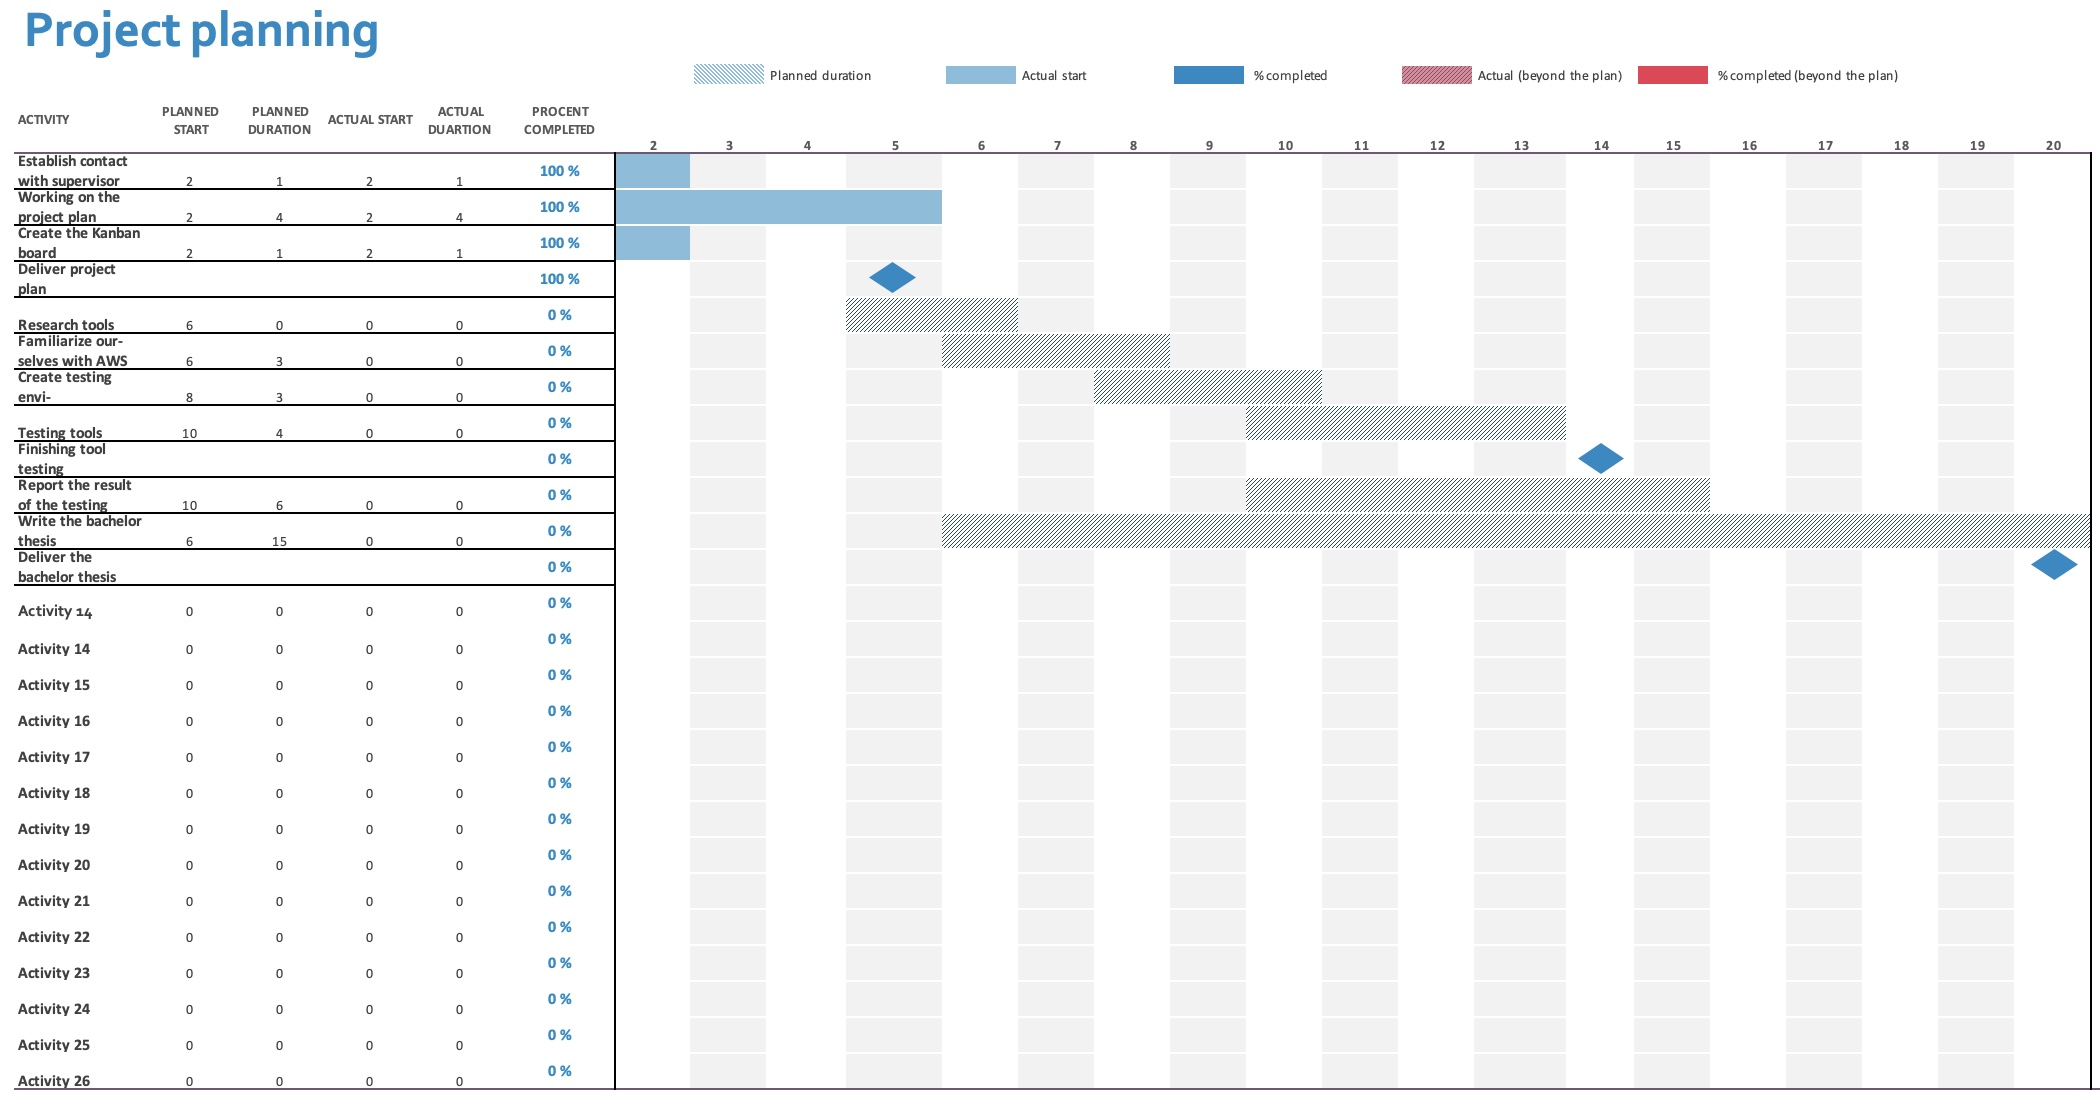
\includegraphics[width=1\columnwidth]{Images/gantt2.jpg}
\\

\newpage

\newpage
\section{Signature}

\begin{tabular}{@{}p{.5in}p{4in}@{}}\\
Approved: & \hrulefill \\
& Anniken Arildset \\
\\
Approved: & \hrulefill \\
& Celina Heimdal Brynildsen \\
\\
Approved: & \hrulefill \\
& Sebastian Hestsveen \\
\\
Approved: & \hrulefill \\
& Thea Urne
\\~\\
\end{tabular}
\newpage


\raggedright 
\printbibliography[heading = bibintoc, title = Bibliography]





